\section{Mobile client}

As described in \cref{sub:smartphone_usage} and \cref{pact}, execution
of an request should be quick and easy to navigate an use, to minimise
the time spend using the system. Throughout this section the
guidelines described in~\cite{DEB} will be followed.

\subsection{Navigation}

Users build mental navigation maps of the systems they are using, and
they tend to keep using already memorised paths to certain views, see
"Box 14.5: How people navigate" \cite{DEB} . \sinote{god citation?
  eller bare referer til bogen?}

First tip to achieve this is that the user should always be able to find \emph{home}, where the user started navigating, from every possible window of the system. This was achieved by having a home button in the top left corner, that always returns to home.

Another tip is to provide a simple and short path to all views. This
was achieved by making all views accessible from home. See \cref{fig:UserInterface}.

\begin{figure}[hbtp]
  \centering
  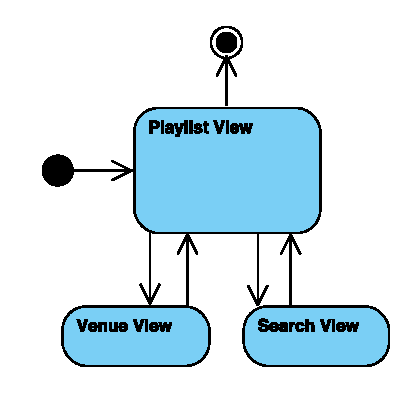
\includegraphics[width=0.5\textwidth]{Images/UserInterface.pdf}
  \caption{Diagram of navigation in the user interface.}\label{fig:UserInterface}
\end{figure}

\begin{itemize}
\item Venue view: The user is presented a list of venues for the user to check in at, see \cref{fig:VenueSketch}.
\item Playlist view: The user is now checked in at a venue and is presented with the playlist of the venue, including what is current playing. See \cref{fig:PlaylistSketch}.
\item Browse view: From here the user can choose a track to add to the playlist from a top- and hot list or make a search query by clicking the magnifyglass. See \cref{fig:BrowseSketch}.
\item Search view: Search results are displayed. These can be added to
  the playlist.
\end{itemize}

When browsing for music in the system, the user is in the procces of
adding to the playlist, therefore navigating to the process adding,
browsing top- and hot lists and searching for a specific track is
grouped as one page visually by a \emph{+} icon. See
\cref{fig:PlaylistSketch}. To ensure that if a user wants to return to
previously requested a search query after pressing home, now the "+"
icon takes them back to their results. Also if the user already did
one search, one might want to do another shortening to path while
maintaining the mental mapping. \sinote{forstår ikke dette. skal omskrives}

Should the user want to change venue, one is checked in at, another list view of venue \enquote{swiped} in from the left. Following the reading direction of left to right, giving a notion of upper layered list of venues, from which the user can change between lower layered playlists.

% \begin{figure}
%   \centering
%   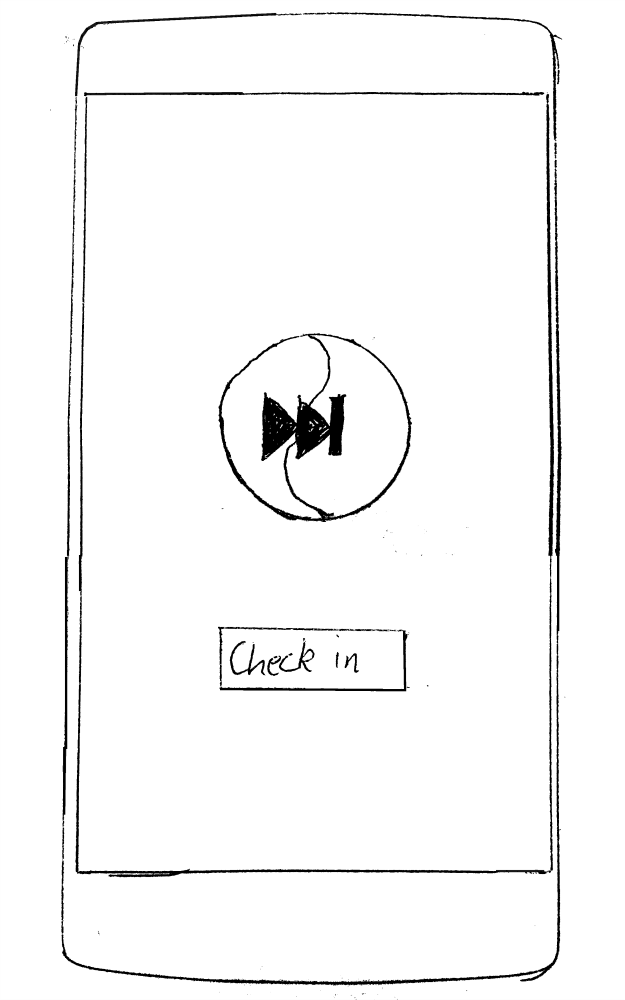
\includegraphics[width=0.25\linewidth]{Images/sketch1.png}
%   \caption{Sketch1}
%   \label{fig:sketch1}
% \end{figure}
% First the user is presented with the systems logo, and a single button. The caption of the button suggest to the user that, one is about to "check in". As shown in \cref{fig:sketch1}.

\begin{figure}[hbtp]
  \centering
  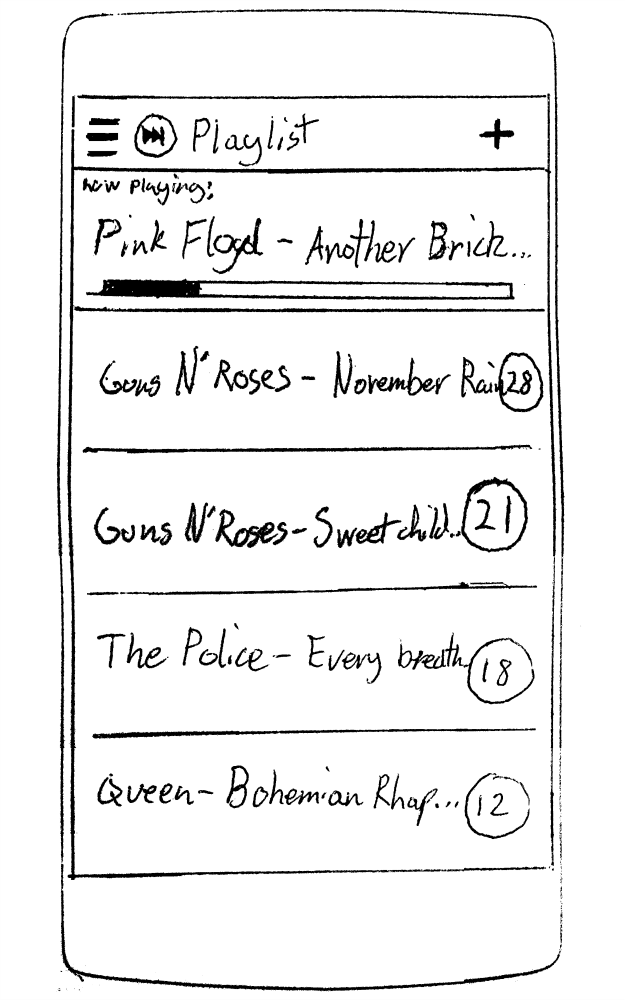
\includegraphics[width=0.3\linewidth]{Images/sketch3.png}
  \caption[Playlist view sketch.]{A "+" icon suggests an action of addition, which in this context is adding to the playlist. If clicked, the user can now browse through tracks and add them to the playlist. The "top" tracks of that specific venue is displayed, or the user can view trending "hot" tracks. Shown in \cref{fig:BrowseSketch}.}
  \label{fig:PlaylistSketch}
\end{figure}

\begin{figure}[hbtp]
  \centering
  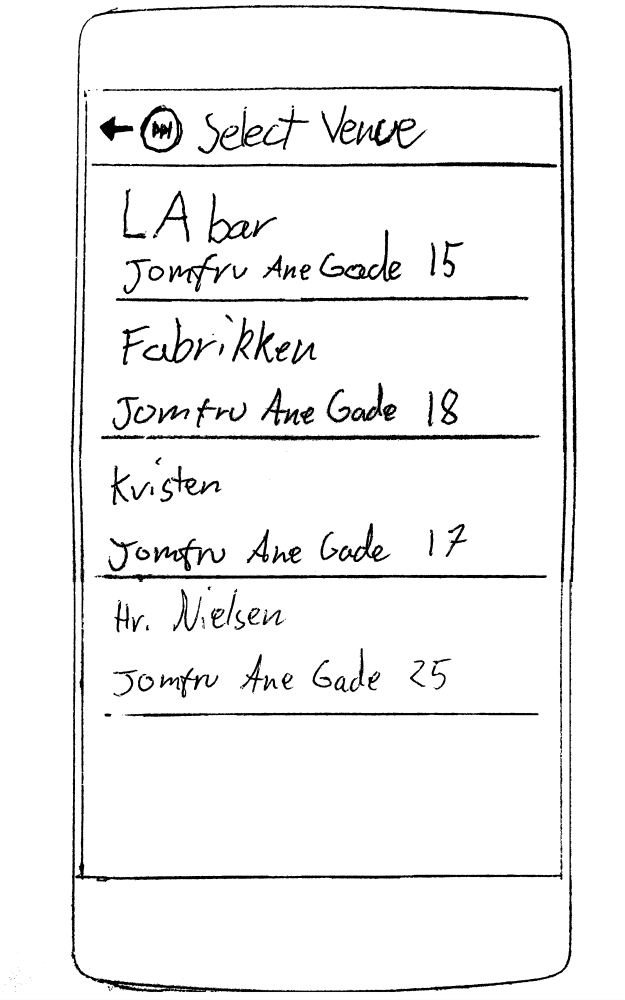
\includegraphics[width=0.3\linewidth]{Images/sketch2.png}
  \caption[Venue view sketch.]{The user can see a listing of nearby open venues. The user can click on any one of these to check in to the venue.}
  \label{fig:VenueSketch}
\end{figure}


\begin{figure}[hbtp]
  \centering
  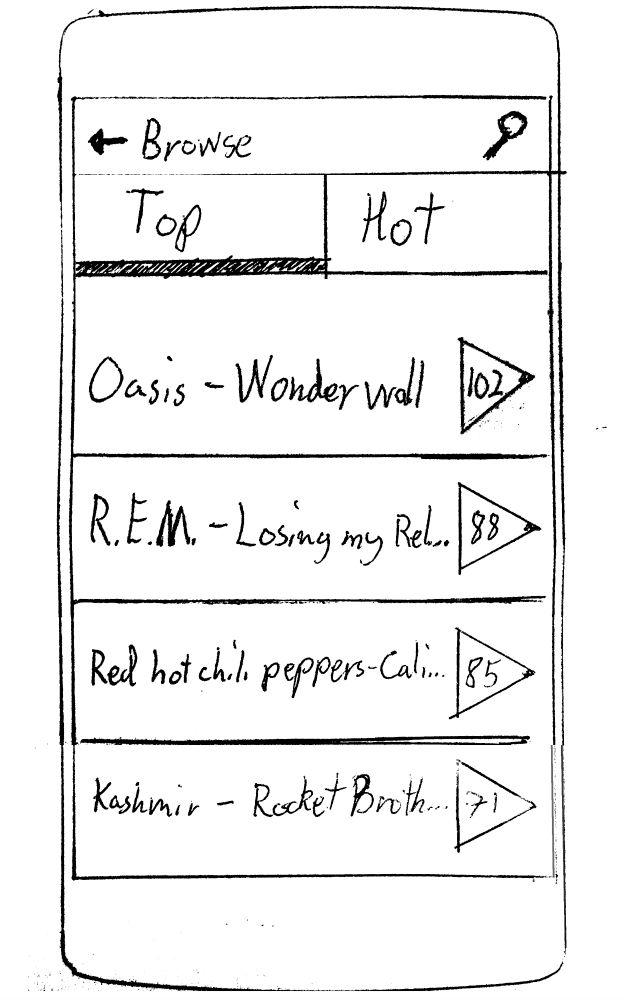
\includegraphics[width=0.3\linewidth]{Images/sketch4.png}
  \caption[Search sketch.]{The magnifying glass at the very top is symbolising an action of searching, when clicked the user can search for specific tracks.}
  \label{fig:BrowseSketch}
\end{figure}

From \cref{sub:usabilityTesting} it was extracted that, the interface should change views automaticly as an confirmation of actions completed. This resulted in when selecting a venue in the venueView or a track in the searchView, the user would be presented with the current playlist of the venue, at the playlistView.
